\chapter{Introduction}

Software systems that exist today are complex and large. As time passes by, these systems get larger and more complex. It is very important that the software systems being developed are more reliable than they were before. For example, if a banking software system is not as reliable as it is supposed to be, then it would not be used by people.
Software development lifecycle has evolved from just developing a software system to developing a robust and reliable software system. Reliability of software depends on its ability to perform all the functions according to the given specifications and to handle the exceptions or abnormal cases [1].
The Design by Contract (DbC) methodology was invented to provide software developers with the ability to construct reliable software systems without much extra effort. DbC has applications throughout the process of building software, from analysis and design to implementation, documentation, debugging and even project management[1]. A contract is made up of pre-conditions and post-conditions which are used for making assertions in the given system. These different conditions define a relationship between a client (end user) and a supplier (software developer). This relationship is said to be broken if any of the conditions do not hold true.



\section{Contract Conditions}

\begin{itemize}
\item A precondition is a condition that should hold true before a call is made to the method. If this condition fails, then the call to the method fails and blame can be assigned to the client for providing incorrect input values.
\item A postcondition is a condition on a method that should hold true when the execution of the method successfully completes. If it does not, then it can be asserted that something went wrong during execution and blame can be assigned to the supplier for providing an erroneous system that does not work according to the given specifications.
\item An invariant condition is something that needs to be true from the start until the end (throughout the execution), of the call to the method.
\end{itemize}

Given these constructs, if an application completes the execution without the failure of any of the pre or post conditions provided in the contract then we can assert that the written code is doing what it is meant for and nothing less or nothing extra [1].
Said this, the quality of the assertion made depends on how well the contracts conditions are written. 

\section{A Contract for ATM System}

An example of a ATM system given below illustrates the use of contract and its constructs.
Here in this example ATM system be our supplier and a person using the ATM system will be the client. Let's suppose supplier provides two functions of depositing and withdrawing money to the client.
\begin{itemize}
\item Withdraw :
Here client is obligated to enter a non-zero amount to be withdrawn from his/her account which also should be less than the balance in his/her account. This obligation for the client forms the precondition of our contract.
Now, once client provides the correct amount to be withdrawn, supplier (ATM system) is obliged to update the balance by decrementing the input amount from it. This obligation for the supplier forms the postcondition of our contract.

\item Deposit :
Here client is obliged to insert the amount to be deposited which should be non-zero and less than the maximum limit allowed (let's say 1500\$). This forms the precondition for the contract of of the Deposit function.
Now, on successful execution of Deposit function, supplier is obliged to increase the balance by the deposited amount. This forms the postcondition of the contract.  
      
\end{itemize}

\section{History ad Background}

Contract Programming also known as Design by Contract (DbC) is one of the methodologies that can be used for software design and development [1]. This methodology was first introduced to the public by Bertrand Meyer as a part of his programming language named Eiffel. Contract Programming was an integral part of Eiffel but the methodology in itself can be used in any language. Fig.~\ref{fig:EiffelContract} shows an example of how contracts are written in Eiffel programming language [2].

\begin{figure}[htb]
\centering
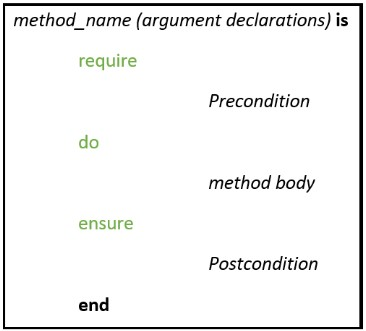
\includegraphics[width=0.5\textwidth]{images/EiffelContract.jpg}
\caption{Contract in Eiffel.} 
\label{fig:EiffelContract}
\end{figure}

Another important aspect of Contract Programming is that it helps build and design a robust and fault tolerant software system, which is why it has been used repeatedly by many developers in the form of libraries or as a language feature.
Contract Programming uses a contract agreed upon by both the developer of the software and the user of the software. In Meyer’s terms, a developer is the supplier and a user is the client [1].  
Here the user of the software must agree and abide to the preconditions that contract specifies. If the user has done so, then method should return the results that satisfy the post-conditions. In this way, when a software system runs into an error state it is very easy for one to detect who is to be blamed. If the problem is with the preconditions, then it is the client who is to be blamed [2]. If the problem is with the results, which means the post-conditions are not met, then the software system has a defect on the side of the supplier. This way it is ensured that the software system does what it is supposed to and that any errors can be easily identified.

